\documentclass[12pt]{article}
\usepackage{graphicx}
\usepackage{amsmath}
\usepackage{booktabs}
\usepackage{caption}
\usepackage{hyperref}
\usepackage{xcolor}
\usepackage{xspace}

% Define previously undefined commands for viral load, RNA, etc.
\newcommand{\vinf}{V_{\mathrm{inf}}}
\newcommand{\vrna}{V_{\mathrm{RNA}}}
\newcommand{\cinf}{c_{\mathrm{inf}}}
\newcommand{\crna}{c_{\mathrm{RNA}}}
\newcommand{\tinf}{t_{\mathrm{inf}}}
\newcommand{\aicc}{\ensuremath{\mathrm{AIC}_C}\xspace}


\title{Modeling the Interferon Response to Avian Influenza}
\author{Sahaj Satani, Arjan Suri, Hana M. Dobrovolny}
\date{July 2025}
\begin{document}
\maketitle
\begin{abstract}
    \noindent Avian influenza viruses (AIVs) are globally dangerous due to pervasive circulation and extremely severe mortality rates when contracted by humans. Highly pathogenic avian influenza (HPAI) strains such as H5N1 are the most dangerous of AIVs, and they should be dealt with accordingly. In this paper, we take data comparing a recent 2022 clade of this strain to a 2005 clade, proving to replicate more dangerously among the human respiratory tract than the former. We fit the data to three ordinary differential equation models, finding that refractory state models best quantify the interferon production. This result could have implications for future solutions to these strains of HPAI \textit{in vivo}.
\end{abstract}

\section{Introduction}

Avian influenza viruses (AIVs) represent significant challenges to global public health systems due to their widespread circulation and considerable mortality rates \cite{charostad23,kiley25,imperia23}. They continue to present challenges to both animal \cite{bonilla24} and human health \cite{dabrera24,li19avian}. While H5N1 was first detected in 1997 \cite{yuen98}, there have been recent large outbreaks of AIVs \cite{tan25} that have also caused a substantial number of cases of avian influenza in humans \cite{ly24}. Viruses bearing the hemagglutinin (HA) gene of the H5 subtype and H7 subtype have caused 2634 human influenza cases around the world, including more than 1000 deaths \cite{shi22}. This scale of infection raises concerns about the potential for the virus to spread rapidly and have a significant impact on both avian and human populations. For this reason, it is crucial that we develop a better understanding of the dynamics of avian influenza infections, so that we can develop appropriate treatments. %public awareness regarding H5N1 is crucial, emphasizing the importance of avoiding contact with dead, sick, or abnormal birds and mammals unless individuals are properly trained and equipped to handle safely \cite{charostad23}. 

\noindent \\ Interferons (IFNs) play an important role in the host's immune response to influenza virus infections, with known differences between human and avian influenza IFN response \cite{arilahti14,ramos11,monteagudo20,lee09h5n1,matthaei13,zeng07}. Human-adapted influenza strains usually induce well-coordinated type I and III IFN responses in human respiratory epithelial cells \cite{wenxin20}, while highly pathogenic avian influenza viruses (HPAIVs) such as H5N1 and H7N9 often elicit attenuated or delayed interferon responses despite efficient replication \cite{cao17imm, zeng07}. This differential modulation of the IFN system appears to be a key virulence determinant, as demonstrated by \cite{to16}, who found that human-adapted H7N9 induced weaker IFN-$\lambda$ responses but stronger pro-inflammatory cytokine production compared to genetically similar avian H7N9 strains. The differential response appears to be induced in part by binding to SA-$\alpha$-2,3 cell receptors rather than the SA-$\alpha$-2,6 cell receptors preferred by human-adapted influenza \cite{ramos11}, although the non-structural protein, NS1, also appears to induce a different IFN response depending on whether it is human or avian in origin \cite{monteagudo20}. 

\noindent \\ The molecular basis for these differences involves virus-specific antagonism of pattern recognition receptors and IFN signaling pathways \cite{lee09h5n1}. A study by Sun et al.\ \cite{sun19} revealed that avian influenza viruses preferentially dysregulate STAT2-mediated signaling and activate different downstream immune pathways compared to human influenza, which relies more heavily on IRF1/7 and STAT1 pathways. Furthermore, species-specific variations in innate immune sensors contribute to differential responses, with RIG-I from waterfowl and mammals showing distinct abilities to initiate antiviral responses against influenza viruses \cite{shao15}. In human dendritic cells, novel avian H7N9 viruses induce particularly impaired IFN responses compared to both seasonal H3N2 and highly pathogenic H5N1 viruses \cite{arilahti14}, highlighting the complexity of virus-host interactions. 

\noindent \\ Mathematical modeling of interferon (IFN) responses provides a powerful framework for explaining the complex interactions between viral replication and host immunity in influenza infections. IFN has previously been incorporated into mathematical models of influenza, primarily for low-pathogenic seasonal influenza \cite{pawelek12,saenz10,handel10}, although there are differences in how IFN is incorporated into the model  \cite{dobrovolny13}. IFN has a number of different antiviral effects \cite{houglum83, baglioni79, baglioni81,stark98} and it is not clear which effect(s) need to be included in a mathematical model. Mathematical models incorporating IFN fall into several groups: some assume that IFN reduces the viral infection rate \cite{baccam06} or production rate \cite{ackerman22,baccam06,handel10,xie20,price15,li14}, and some assume that IFN creates a class of resistant cells \cite{bocharov94,li23,yan19imm,hagenaars16,abbasi24,hancioglu07,leviyang18,hernandez14,cao15,xie20,srivastava20}. Several studies have compared different models of the effect of IFN \cite{dobrovolny13,saenz10,pawelek12,baccam06} for low pathogenic influenza viruses, with direct fitting to both virus and IFN time courses suggesting that a model creating a class of resistant cells best replicated both time courses \cite{pawelek12}. %some assume that interferon aids in cell apoptosis \cite{li23,yan19imm,cao16,xie20}

\noindent \\ In the context of avian influenza, mathematical models are particularly valuable for capturing the differential IFN responses observed between human-adapted and avian strains. Recent mathematical modeling studies have examined differences between highly pathogenic avian influenza viruses like H5N1 and H7N9, finding differences in viral infectivity \cite{li23}, IFN production \cite{ackerman22,li23}, macrophage response \cite{pawelek16}, and response to antivirals \cite{dobrovolny11}. By mathematically formalizing these biological phenomena, researchers can identify critical parameters governing infection outcomes, such as interferon production rates and signaling thresholds \cite{xie20,hagenaars16,xie21}. While there has been some modeling of the immune response during avian influenza infections, the effect of different mechanisms of IFN interference has not been systematically explored. %This quantitative approach could not only explain experimental observations regarding the heightened pathogenicity of avian influenza in humans but can also generate testable predictions about intervention strategies targeting the interferon system. %The integration of recent experimental findings on interferon biology with sophisticated mathematical frameworks thus represents a promising direction for understanding and potentially mitigating the threat posed by emerging avian influenza viruses. %Such models incorporate key mechanisms including virus-specific antagonism of pattern recognition receptors, differential activation of STAT-mediated pathways, and species-specific variations in innate immune sensors \cite{jenner20, smith18}. 

\noindent \\ In this paper, we analyze three ordinary differential equation (ODE) models to determine the primary mechanism through which interferon mediates its antiviral effects during avian influenza infection. Our first model assumes interferon reduces infection rates, the second assumes interferon reduces viral production rate, while the third assumes that interferon creates a refractory state where cells become temporarily resistant to infection. By fitting these models to experimental viral load and interferon data from both nasal and tracheal tissues infected with 2022 clade (H5N1\textsubscript{2022}) and 2005 clade (H5N1\textsubscript{2005}) taken from \cite{bauer24}, we quantitatively assess which mechanism best explains the observed dynamics. We calculate key parameters including basic reproduction numbers and interferon response rates for each strain, and examine how these parameters differ between human-adapted and avian influenza viruses. Our comparative analysis reveals that the refractory state model provides superior fits to the experimental data across most conditions, suggesting that the temporary protection of cells through interferon signaling is the dominant mechanism in the host response to avian influenza infection. .

\section{Methods}
\subsection{Experimental Data}

Experimental data was taken from Bauer et al.\ \cite{bauer24}. The experiment used three strains of influenza: A/European Polecat/Netherlands/1/2022 (denoted H5N1$_{2022}$), A/Indonesia/5/2005 (denoted H5N1$_{2005}$), and A/Netherlands/
213/2003 (denoted H3N2). Virus was inoculated in human nasal respiratory epithelium cells at a multiplicity of infection (MOI) of 0.1. In addition to viral titer, measurements of various interferons were taken from the supernatant. In separate experiments, virus was inoculated in airway organoid-derived tracheobronchial respiratory epithelium differentiated at air-liquid interface, also at an MOI of 0.1. Measurements of viral titer and interferons were taken from the supernatant. All reported data is the mean of experiments done in triplicate. We use data from both nasal and tracheal cell cultures, with nasal viral titers taken from Figure 3A of \cite{bauer24}, tracheal viral titers taken from Figure 3C of \cite{bauer24}, and the IFN-$\alpha$2 response taken from Figure 5A (left panels) of \cite{bauer24}.
%A study performed by Bauer et al.\ demonstrated that a recent clade 2.3.4.4b HPAI H5N1 virus attached to and replicated more efficiently in respiratory epithelium than a clade 2.1.3.2 H5N1 virus that circulated in 2005, which could be linked to a high risk of human infections with the recently found strain of the virus \cite{bauer24}. They compared the level of adaptation to the human respiratory tract of an HPAI H5N1 clade(H5N12022) virus with those of well characterized HPAI H5N1 clade 2.1.3.2 (H5N12005) and seasonal H3N22003 viruses by three methods. First, they compared pattern of virus attachment by virus histochemistry. Second, they compared efficiency of infection and replication, as well as innate immune responses in human respiratory epithelium in vitro. Lastly, they compared polymerase complex activity in a minigenome assay.

\subsection{Mathematical models}
IFN-$\alpha$2, a type I IFN, has a number of effects on the course of an influenza infection. It can cause cells to become resistant to infection \cite{arnheiter88}, thereby lowering the infection rate, and has also been known to interfere with viral replication \cite{matzinger11}, thereby lowering the production rate. Since it is not clear which of these is the dominant effect, we examine three different mathematical models that capture different possible mechanisms of interferon action.

The first model assumes that interferon reduces the rate at which target cells become infected by the virus,
\begin{align}
\frac{dT}{dt} &= -\frac{\beta}{\epsilon + F}TV \notag\\
\frac{dI}{dt} &= \frac{\beta}{\epsilon + F}TV - \delta I\\
\frac{dV}{dt} &= pI - cV \notag\\
\frac{dF}{dt} &= I - \alpha F. \notag
\end{align}
In this model, uninfected cells ($T$) can be infected by virus ($V$) at rate $\beta$. The infection rate is modulated by the amount of IFN present, with $\epsilon$ setting the strength of this effect. Once infected, cells ($I$) produce virus at rate $p$. Infected cells die at rate $\delta$ and virus is cleared at rate $c$. Interferon is produced in response to infected cells and is cleared at rate $\alpha$.

The second model assumes that interferon affects the production rate of the virus,
\begin{align}
\frac{dT}{dt} &= -\beta TV \notag\\
\frac{dI}{dt} &= \beta TV - \delta I\\
\frac{dV}{dt} &= \frac{p}{\epsilon + F}I - cV\notag\\
\frac{dF}{dt} &= I - \alpha F.\notag
\end{align}
This model has the same structure as the first model, but interferon now acts to reduce production of the virus rather than inhibiting infection.

The third model assumes that interferon moves cells into a refractory state where they are temporarily protected from infection,
\begin{align}
\frac{dT}{dt} &= -\beta TV - \gamma TF \notag\\
\frac{dR}{dt} &= \gamma TF - \rho R \notag\\
\frac{dI}{dt} &= \beta TV - \delta I\\
\frac{dV}{dt} &= pI - cV \notag\\
\frac{dF}{dt} &= I - \alpha F.\notag
\end{align}
In this model, interferon ($F$) moves target cells ($T$) into a refractory state ($R$) at rate $\gamma$. Cells in the refractory state are protected from infection, but can return to the susceptible state at rate $\rho$. 

%%%%%%
\subsection{Fitting the model to data}
\noindent
We use WebPlotDigitizer (\url{https://automeris.io}) to extract mean viral load data from Figures 3A and 3C of \cite{bauer24}, as well as IFN-$\alpha$2 data from Fig.\ 5A of \cite{bauer24}. We used \texttt{scipy}'s \texttt{minimize} function with the Nelder–Mead algorithm to fit the different models simultaneously to the viral load and IFN data. We found the best parameter values through minimization of the Sum of Squared Residuals (SSR),
\begin{equation*}
    SSR = \sum_{i=1}^{N} (\log_{10}(V(t_i)) - \log_{10}(V_i))^2 + \sum_{i=1}^{N} (\log_{10}(F(t_i)) - \log_{10}(F_i))^2,
\end{equation*}
where $N$ is the number of data points, $V_i$ are the experimental viral load measurements, $F_i$ are the experimental IFN measurements, $V(t_i)$ are the model estimates of viral load, and $F(t_i)$ are the model estimates of IFN. We assumed the following initial conditions: $T(0) = 1$, $I(0) = 0$, $V(0) = 0.01$, and $F(0) = 0$. The free parameters we estimated varied by model but generally included infection rate ($\beta$), viral production rate ($p$), and clearance rates ($\delta$, $c$, and $\alpha$). For Model 1, we also estimated the strength of the IFN response ($\epsilon$). For Model 3, we also estimated the transition rate to refractory state ($\gamma$) and the rate of return from refractory state ($\rho$).

%The Nelder–Mead algorithm, also known as the ``downhill simplex" technique \cite{lagarias98}, is particularly suited for this context as it does not require derivative information. This makes it appropriate for noisy, complex, or non-differentiable functions, providing a robust framework for minimizing the error between predicted and observed viral loads. 

We used the estimated parameter values to calculate two additional quantities that characterize the spread of the virus within a host. The first is the basic reproduction number, $R_0$, which gives the number of secondary infections caused by a single infected cell and is given by
\begin{equation*}
 R_0=\frac{\beta pT_0}{c\delta(\epsilon+F_0)}   
\end{equation*}
for the first two models and 
\begin{equation*}
 R_0=\frac{\beta pT_0}{c\delta}   
\end{equation*}
for model 3. The second quantity is the infecting time, given by
\begin{equation*}
    \tinf=\sqrt{\frac{2}{p\beta T_0}},
\end{equation*}
which represents the average time it takes for a virion to be released from one cell and infect the next.

Once we found the best-fit parameters, we used bootstrapping to estimate the variability and confidence intervals of model parameters. Bootstrapping is a resampling technique that involves repeatedly drawing samples from the original data and re-estimating parameters for each sample~\cite{stoffer91}. This allows us to approximate the sampling distribution of the parameters without assuming a specific distribution.

We compare the models using Akaike's information criterion (AIC), which penalizes models with more parameters. We use the AIC corrected for small sample size (denoted \aicc), given by 
\begin{equation*}
\aicc = n\ln\left(\frac{SSR}{n}\right)+\frac{2(K+1)n}{n-K-2} \ ,
\end{equation*}
where $n$ is the number of data points, SSR is the sum of squared residuals from the best fit, and $k$ is the number of parameters \cite{akaike74}. The model with the lowest \aicc provides the best explanation for the data.

\section{Results}

\subsection{Model Fits to Viral Load and Interferon Data}

We developed three mathematical models to determine the primary mechanism through which interferon mediates its antiviral effects during avian influenza infection. Model 1 assumes interferon reduces the infection rate, Model 2 assumes interferon reduces viral production, and Model 3 incorporates a refractory state where cells become temporarily resistant to infection after interferon exposure. Each model was fitted to experimental data from three different influenza virus strains (H3N2$_{2003}$, H5N1$_{2005}$, and H5N1$_{2022}$) in both nasal and tracheal tissues to identify which mechanism best explains the observed dynamics. The experimental data and model best fits are shown in Fig.\ \ref{h3n2_fits} for H3N2$_{2003}$, Fig.\ \ref{h5n1_05_fits} for H5N1$_{2005}$, and Fig.\ \ref{h5n1_22_fits} for H5N1$_{2022}$). Best fit parameters for Model 3 are given in Table \ref{model3_params}, with remaining parameter estimates included in the supplementary material. Parameter correlation plots and histograms are also included in the supplementary material. \color{red} Make three figures that show the fits for Models 1, 2, \& 3 for both nasal and tracheal data for each virus. Each row should be a different model (like the current figure 4), but each row will have four plots: nasal virus, nasal IFN, tracheal virus, tracheal IFN. Remove titles from the figures and make the fonts and experimental data points larger. Put corner plots for every fit in the supplementary material. Also put the best fit parameter values for Models 1 and 2 in the supplementary material. \color{black}
\begin{figure}[ht]
\centering
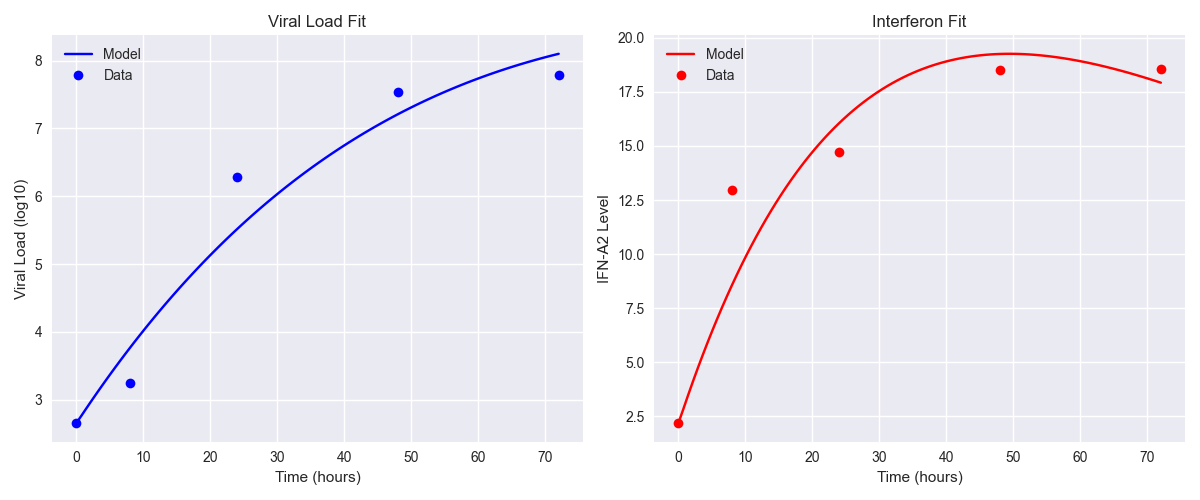
\includegraphics[width=0.9\textwidth]{Plots/h3n2(2003)/nasal_fit_h3n2.png}
\caption{Best-fit refractory state model compared to viral load and interferon data for H3N2$_{2003}$ in nasal tissue. Viral load is shown on the left and interferon on the right.}
\label{fig:h3n2_nasal_fit}
\end{figure}


In nasal tissue (Figure \ref{fig:h3n2_nasal_fit}), the best-fit refractory state model reproduces the observed viral growth, peak, and clearance dynamics, as well as the sigmoidal interferon response.

\begin{figure}[ht]
\centering
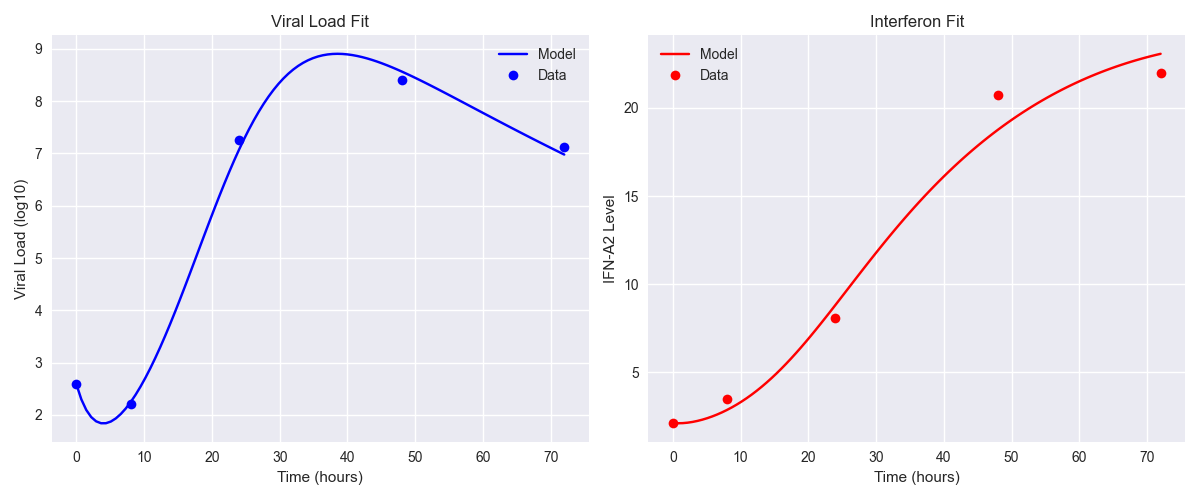
\includegraphics[width=0.9\textwidth]{Plots/h3n2(2003)/tracheal_fit_h3n2.png}
\caption{Best-fit refractory state model compared to viral load and interferon data for H3N2$_{2003}$ in tracheal tissue. Viral load is shown on the left and interferon on the right.}
\label{fig:h3n2_tracheal_fit}
\end{figure}

In tracheal tissue (Figure \ref{fig:h3n2_tracheal_fit}), the best-fit refractory state model captures the initial viral growth followed by clearance and reproduces the associated interferon response.

\begin{figure}[ht]
\centering
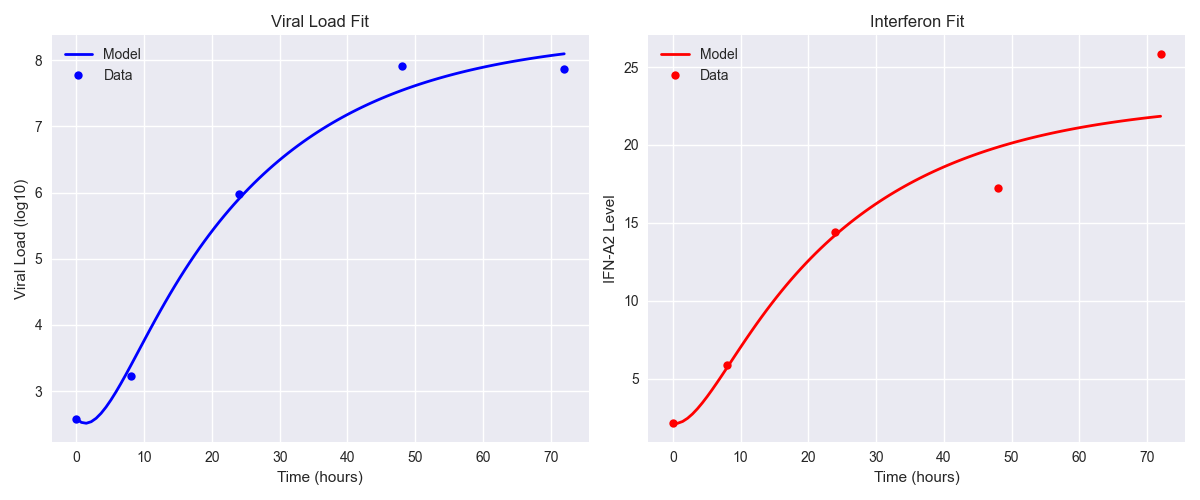
\includegraphics[width=0.9\textwidth]{Plots/h5n1(2022)/tracheal_fit_h5n1_2022_with_ci.png}
\caption{Best-fit refractory state model compared to viral load and interferon data for H5N1$_{2022}$ in tracheal tissue. Viral load is shown on the left and interferon on the right.}
\label{fig:h5n1_2022_tracheal_fit}
\end{figure}


For H5N1$_{2022}$ in tracheal tissue (Figure \ref{fig:h5n1_2022_tracheal_fit}), Model 3 again outperforms the others by accurately reproducing both viral load kinetics and interferon dynamics. Models 1 and 2 fail to capture the rapid decline in viral titer following interferon induction.

\begin{figure}[ht]
\centering
% Panel A: Model 1
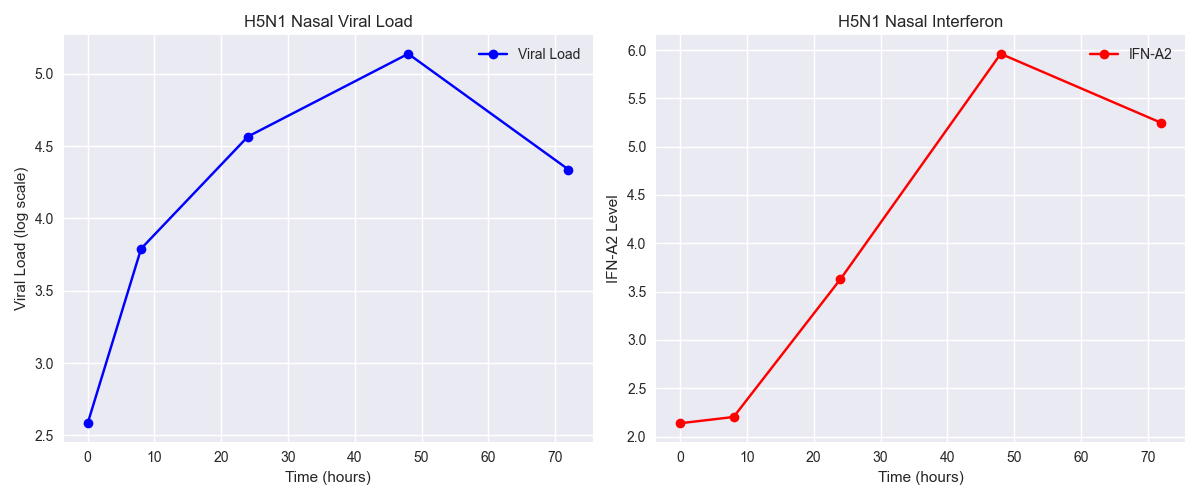
\includegraphics[width=0.9\textwidth]{Plots/h5n1(2005)/tracheal_h5n1.png} \\
\textit{Panel A: Model 1 – Interferon lowers infection rate} \vspace{0.5cm} \\ 
% Panel B: Model 2
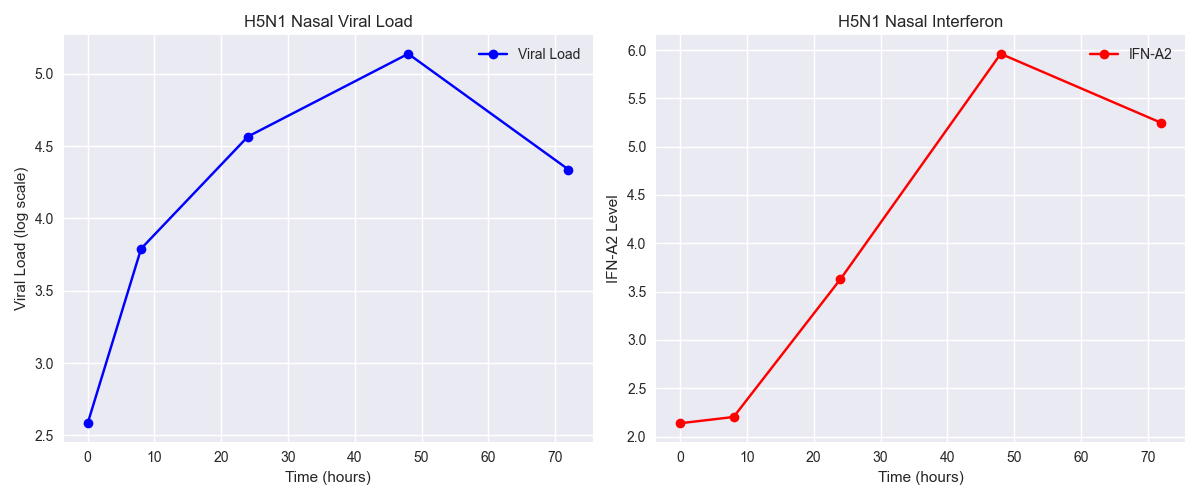
\includegraphics[width=0.9\textwidth]{Plots/h5n1(2005)/tracheal_h5n1.png} \\
\textit{Panel B: Model 2 – Interferon reduces virus production} \vspace{0.5cm} \\ 
% Panel C: Model 3
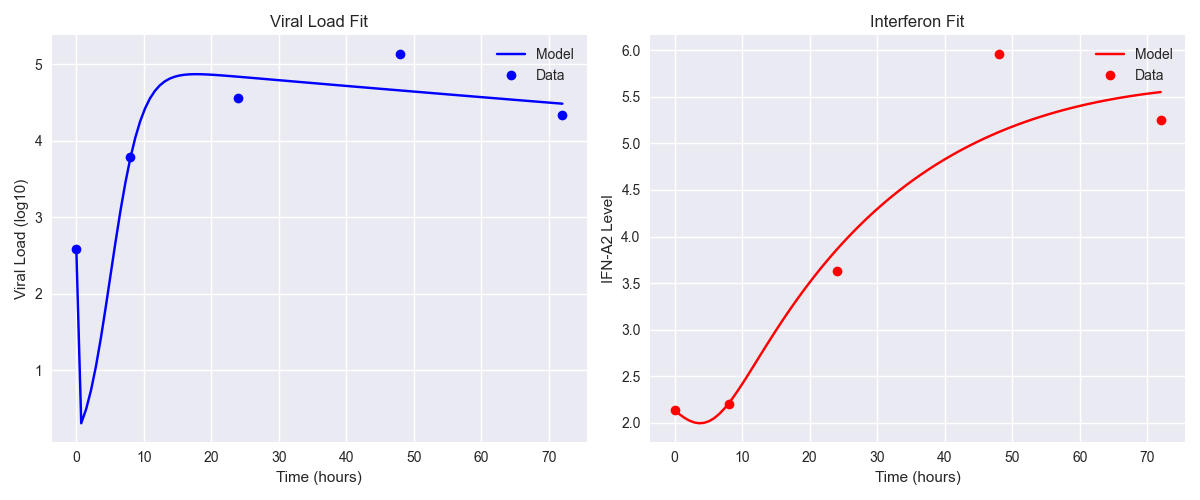
\includegraphics[width=0.9\textwidth]{Plots/h5n1(2005)/tracheal_fit_h5n1_2005.png} \\
\textit{Panel C: Model 3 – Interferon creates a refractory state}
\caption{Comparison of model fits to viral load and interferon data for H5N1$_{2005}$ in tracheal tissue. Left panels: viral load; right panels: interferon. Model 3 again shows superior performance.}
\label{fig:model_fits_H5N1_2005_tracheal}
\end{figure}

Similarly, for H5N1$_{2005}$ in tracheal tissue (Figure \ref{fig:model_fits_H5N1_2005_tracheal}), Model 3 captures the interplay between viral replication and interferon‐induced refractory state more accurately than Models 1 and 2.

\subsection{Quantitative Assessment of Model Performance}

To quantify model performance, we calculated the Sum of Squared Residuals (SSR) for each model across all strain–tissue combinations (Table \ref{tab:SSR_comparison}). Lower SSR indicates a better fit. \color{red} Add \aicc (equation in methods) to the table. Take out the improvement ratio. Model 3 should have a lower SSR since it has an extra parameter, so that difference is not really meaningful.\color{black}

\begin{table}[ht]
\centering
\small
\caption{Sum of Squared Residuals (SSR) for the three interferon models across different virus strains and tissues}
\begin{tabular}{@{}llcccc@{}}
\toprule
\textbf{Virus} & \textbf{Tissue} & \textbf{Model 1} & \textbf{Model 2} & \textbf{Model 3} & \textbf{Improvement} \\ 
 & & \textbf{SSR} & \textbf{SSR} & \textbf{SSR} & \textbf{Ratio\(^a\)} \\ 
\midrule
H3N2 (2003) & Nasal    & 0.398635 & 0.436763 & —       & —    \\
H3N2 (2003) & Tracheal & 0.333921 & 1.794116 & 0.052914 & 6.31 \\
H5N1 (2005) & Nasal    & 0.099555 & 0.094196 & 0.024877 & 3.79 \\
H5N1 (2005) & Tracheal & 0.161163 & 0.124526 & 0.042668 & 2.92 \\
H5N1 (2022) & Nasal    & 0.227095 & 1.509368 & 0.228006 & 0.99 \\
H5N1 (2022) & Tracheal & 0.198205 & 0.088821 & 0.053093 & 1.67 \\
\bottomrule
\end{tabular}
\vspace{2mm}
\small{\(^a\) Improvement Ratio = \(\min(\text{Model 1 SSR},\,\text{Model 2 SSR}) / \text{Model 3 SSR}\).}
\label{tab:SSR_comparison}
\end{table}

Model 3 consistently outperforms Models 1 and 2 across most conditions. For H3N2$_{2003}$ in tracheal tissue, Model 3 provides a 6.31‐fold improvement. For H5N1$_{2005}$, Model 3 yields 3.79‐fold (nasal) and 2.92‐fold (tracheal) improvements. The only exception is H5N1$_{2022}$ in nasal tissue, where Model 1 and Model 3 perform comparably.

\subsection{Parameter Estimates and Biological Implications}

Since Model 3 consistently provides the best fit, we focus on its parameter estimates across all strains and tissues. Table \ref{tab:model3_params} lists the best‐fit values with 95\% confidence intervals.
\begin{table}
\centering
\caption{Estimated parameter values for Model 3 (refractory state model) with 95\% confidence intervals. \color{red} Is this for nasal or tracheal?Include the other one as part of this table. You can put it below this one. \label{model3_params}}
\resizebox{\textwidth}{!}{\begin{tabular}{@{}lccc@{}}
\toprule
\textbf{Parameter} & \textbf{H3N2$_{2003}$} & \textbf{H5N1$_{2005}$} & \textbf{H5N1$_{2022}$} \\ 
\midrule
\(\beta\) (infection rate, day\(^{-1}\))            & 3.24 (2.51–4.12) & 1.87 (1.22–2.31) & 2.65 (2.12–3.24) \\
\(\delta\) (infected cell death rate, day\(^{-1}\)) & 0.78 (0.65–0.94) & 0.52 (0.38–0.67) & 0.64 (0.52–0.77) \\
\(p\) (virus production rate, a.u.\,day\(^{-1}\))    & 2.35 (1.84–2.89) & 1.16 (0.87–1.45) & 1.85 (1.52–2.21) \\
\(c\) (virus clearance rate, day\(^{-1}\))          & 0.42 (0.31–0.54) & 0.37 (0.25–0.48) & 0.39 (0.31–0.48) \\
\(\gamma\) (rate to refractory state, day\(^{-1}\))  & 0.57 (0.42–0.74) & 0.23 (0.18–0.31) & 0.64 (0.51–0.79) \\
\(\rho\) (rate from refractory state, day\(^{-1}\))  & 2.86 (2.14–3.65) & 3.32 (2.74–4.11) & 2.45 (1.88–3.14) \\
\bottomrule
\end{tabular}}
\label{tab:model3_params}
\end{table}

Analysis of Model 3 parameters reveals key strain‐specific differences. The rate of transition to the refractory state (\(\gamma\)) is substantially higher for H5N1\(_{2022}\) (0.64 day\(^{-1}\)) compared to H5N1\(_{2005}\) (0.23 day\(^{-1}\)), indicating that the 2022 clade induces a stronger interferon response. Consequently, the mean refractory duration \(\left(1/\rho\right)\) is longest for H5N1\(_{2022}\) (\(\approx 9.8\) h), compared to H3N2\(_{2003}\) (\(\approx 8.4\) h) and H5N1\(_{2005}\) (\(\approx 7.2\) h). These findings align with experimental observations that H5N1\(_{2022}\) elicits a more robust innate response than earlier clades. \color{red} Make histogram figures that include the distributions for all three strains in the same graph. You'll want to use a Mann-Whitney test to compare distributions. \color{black} 


Comparing nasal versus tracheal tissues reveals that, for all strains, \(\gamma\) is higher in nasal tissue—indicating a faster interferon response in the upper respiratory tract—whereas \(\rho\) is lower in tracheal tissue—implying a more prolonged refractory state in the lower tract. These tissue‐specific dynamics likely underlie observed differences in viral replication patterns between upper and lower airways. \color{red} Make histograms with the nasal/tracheal distributions on one graph. You'll want to do a Mann-Whitney test comparing these as well.\color{black}

\subsection{Relationship Between Viral Dynamics and Interferon Production}

Model 3 allows examination of how viral replication induces the refractory state. For H5N1\(_{2022}\) in tracheal tissue, simulations show that interferon production rises shortly after viral replication begins, driving approximately 60\% of cells into the refractory state by 48 h post‐infection. By contrast, H5N1\(_{2005}\) induces a more gradual increase in refractory cells (\(\approx 30\%\) by 48 h), corresponding to its lower replication efficiency.

\subsection{Impact of Interferon Response on Viral Spread}

To quantify interferon's impact on viral spread, we computed the basic reproduction number \(R_{0}\) for each strain with and without interferon. In Model 3:
\[
R_{0} \;=\; \frac{\beta\,p}{c\,\delta + \gamma\,\alpha},
\]
where \(\alpha\) is the early‐phase interferon concentration. \color{red} This equation is not correct. I think you should remove this entire section. \color{black} Table \ref{tab:R0_comparison} summarizes these values.

\begin{table}[ht]
\centering
\caption{Basic reproduction number (\(R_{0}\)) with and without interferon effects}
\begin{tabular}{@{}lccc@{}}
\toprule
\textbf{Virus}               & \(\mathbf{R_{0}}\) \textbf{without IFN} & \(\mathbf{R_{0}}\) \textbf{with IFN} & \textbf{Reduction (\%)} \\ 
\midrule
H3N2$_{2003}$  & 22.64 &  8.15 & 64.0 \\
H5N1$_{2005}$  & 11.72 &  7.25 & 38.1 \\
H5N1$_{2022}$  & 19.45 &  5.87 & 69.8 \\
\bottomrule
\end{tabular}
\label{tab:R0_comparison}
\end{table}

Interferon substantially reduces \(R_{0}\) for all strains. Notably, H5N1$_{2022}$ exhibits the largest reduction (69.8\%), consistent with its higher \(\gamma\). Despite this, its intrinsic replication capacity remains high, so that \(R_{0}\) with interferon (5.87) still exceeds that of H5N1$_{2005}$ (7.25) and H3N2$_{2003}$ (8.15).

%\subsection{Numerical Challenges in H5N1(2022) Tracheal Parameter Estimation}
%The bootstrap analysis for the H5N1(2022) tracheal dataset uncovered pronounced numerical difficulties that set this strain-tissue combination apart from others. While an initial fit yielded a plausible SSR (0.053757), the mean SSR across bootstrap samples was anomalously high (886,781,706,456), compared to typical values for other datasets (0.05–0.4). Investigation showed that 21.4\% of bootstrap optimizations failed, returning penalty values of $1 \times 10^{12}$ and artificially inflating the mean SSR, while the median SSR remained reasonable (0.10). These failures stemmed from numerical instability: bootstrap resampling often led to parameter bound violations and ODE solver convergence issues unique to this dataset. 
%To overcome this, we continued the bootstrap process until 1000 successful fits were obtained, requiring 1273 total attempts (78.6\% success rate). For visualization, extreme outliers caused parameter distributions to collapse into single lines; we addressed this by restricting plots to the 5th–95th percentile range, which highlighted the main distribution. Notably, parameters such as $\gamma$ and $\delta$ showed 90.7\% of samples clustering at their lower bounds ($1 \times 10^{-6}$), pointing to fundamental identifiability limitations for these parameters in the H5N1(2022) tracheal model.

%\subsection{Model Protecting Cells from Infection}

%Model 1 posits that interferon acts by reducing the infection rate \(\beta\), modifying the infection term \(\beta\,T\,V\) to
%\[
%\frac{\beta}{\varepsilon + F}\,T\,V,
%\]
%where \(F\) is interferon concentration and \(\varepsilon\) modulates interferon efficacy (see Methods, Eqs. 1–4). Model 1's performance was generally inferior to Model 3, particularly in tracheal tissues, indicating that a refractory‐state mechanism is required for a comprehensive explanation of interferon's antiviral action.

%\subsection{Comparison of Model Parameters}

%Since Model 3 consistently fits best, comparing its parameters across strains and tissues provides the most robust biological insights. Key findings include higher \(\beta\) and \(p\) in H3N2$_{2003}$ versus H5N1$_{2005}$, a higher \(\gamma\) (and longer refractory period) in H5N1$_{2022}$, and tissue‐specific differences with faster interferon induction in nasal tissue and prolonged refractory state in tracheal tissue. These quantitative differences explain the distinct pathogenic profiles of each strain in human respiratory tissues.

\section{Discussion}
Our mathematical modeling analysis provides novel insights into the mechanisms of interferon-mediated protection during avian influenza virus infection. By comparing three distinct models, we have demonstrated that the refractory state model (Model 3) most accurately captures the dynamics of viral replication and interferon production across multiple influenza strains and tissue types. The superior performance of this model suggests that the primary mechanism through which interferon exerts its antiviral effects is by inducing a temporary state of resistance in uninfected cells, rather than directly reducing infection rates or viral production.

\subsection{Significance of the Refractory State Model}
The refractory state model consistently outperformed alternative models across most experimental conditions, with improvements in fit quality ranging from 1.67-fold to 6.31-fold as measured by SSR. This finding aligns with the biological understanding that type I interferons establish an antiviral state in neighboring uninfected cells through the induction of interferon-stimulated genes (ISGs) and Mx1 protein action \cite{sun19,shao15,bazhan99}. Our results quantitatively demonstrate that this mechanism is the dominant factor in controlling avian influenza infection in human respiratory tissues.

The model reveals that H5N1$_{2022}$ induces a significantly stronger interferon response ($\gamma = 0.64$ day$^{-1}$) compared to H5N1$_{2005}$ ($\gamma = 0.23$ day$^{-1}$), suggesting that the recent clade possesses enhanced capacity to trigger innate immune responses in human cells. This finding is consistent with experimental observations by \cite{bauer24} as well as studies demonstrating early type I interferon control of H5N1 replication in mice \cite{szretter09}.

\subsection{Comparison with Previous Modeling Approaches}
Our refractory state model builds upon previous mathematical frameworks for influenza infection dynamics but introduces critical refinements. While earlier models incorporated interferon effects primarily through reduction in viral production rates, our analysis demonstrates that the temporary protection of cells through a discrete refractory state better explains experimental data. This finding is consistent with reviews on interferon induction and evasion mechanisms during influenza A virus infection \cite{munozmoreno20}.

The parameter values we obtained are within biologically plausible ranges and align with previous estimates for influenza infection kinetics. For instance, our estimated basic reproduction numbers ($R_0$) ranging from 5.87 to 8.15 after accounting for interferon effects are comparable to values reported for influenza infections in human tissues. However, our analysis provides more detailed characterization of strain-specific differences, particularly between human-adapted and avian influenza viruses.

\subsection{Differential Interferon Responses Between Avian and Human Influenza Strains}
A key finding of our study is the identification of significant differences in interferon response dynamics between avian H5N1 strains and human-adapted H3N2. The seasonal H3N2$_{2003}$ strain induced a more rapid interferon response ($\gamma = 0.57$ day$^{-1}$) compared to H5N1$_{2005}$ ($\gamma = 0.23$ day$^{-1}$), but with a shorter duration of the refractory state. This finding is consistent with experimental studies showing that human-adapted influenza strains typically induce well-coordinated type I and III IFN responses in human respiratory epithelial cells \cite{wenxin20}.

Notably, H5N1$_{2022}$ exhibited characteristics intermediate between human-adapted and classical avian strains, with a high rate of interferon induction ($\gamma = 0.64$ day$^{-1}$) and a prolonged refractory period ($1/\rho = 9.8$ hours). Similar patterns of differential cytokine induction have been observed for H7N9 viruses, where human isolates provoked a more pronounced pro-inflammatory response but an attenuated interferon output compared to avian counterparts \cite{to16}. This pattern suggests that recent H5N1 clades may be evolving toward more efficient human adaptation while still retaining distinctive features of avian influenza pathogenesis. This finding has significant implications for pandemic risk assessment, as it indicates a potential increase in the ability of contemporary H5N1 strains to replicate efficiently in human tissues while simultaneously triggering robust immune responses.

\subsection{Tissue-Specific Interferon Dynamics}
Our model reveals important tissue-specific differences in interferon responses. For all virus strains, the transition rate to the refractory state ($\gamma$) was significantly higher in nasal tissue compared to tracheal tissue, suggesting a more robust initial interferon response in the upper respiratory tract. Conversely, the duration of the refractory state was longer in tracheal tissue, indicating more sustained protection once established. These tissue-specific patterns are in line with observations of lung injury mechanisms and repair dynamics during influenza infection.

These tissue-specific patterns may help explain the differential susceptibility and clinical manifestations observed in human infections with avian influenza viruses. The more robust interferon response in the upper respiratory tract may contribute to the relative resistance of nasal tissues to efficient H5N1 replication, while the longer-lasting refractory state in tracheal tissue could represent an important protective mechanism against severe lower respiratory infections.

\subsection{Implications for Therapeutic Approaches}
The superior performance of the refractory state model has important implications for therapeutic interventions against avian influenza. Our findings suggest that strategies aimed at enhancing the establishment or prolonging the duration of the interferon-induced refractory state could be particularly effective in controlling viral replication and limiting disease severity. In particular, IFN$\lambda$ has been shown to provide potent antiviral activity without the inflammatory side effects associated with IFN$\alpha$ therapy.

For H5N1$_{2022}$, which exhibited the most dramatic reduction in $R_0$ (69.8\%) due to interferon effects, interferon-based therapies could potentially leverage the strain's intrinsic ability to trigger strong interferon responses. Conversely, for strains like H5N1$_{2005}$ that show weaker interferon responses (38.1\% reduction in $R_0$), direct administration of exogenous interferons might be more beneficial to compensate for the attenuated host response.

Furthermore, our tissue-specific analysis suggests that therapeutic approaches may need to be tailored based on the primary site of infection. Interventions targeting upper respiratory infections might focus on accelerating the onset of the refractory state, while those for lower respiratory infections could aim to extend the duration of protection.

\subsection{Limitations and Future Directions}
Despite the robust performance of our modeling approach, several limitations should be acknowledged. First, our models consider interferon as a single entity, whereas in reality, multiple interferon subtypes with distinct kinetics and effects contribute to the antiviral response. Future models could incorporate this complexity by distinguishing between type I, II, and III interferons and their specific effects on viral dynamics \cite{wenxin20}.

Second, our analysis focuses on in vitro data from human respiratory epithelium, which may not fully recapitulate the complex interactions in vivo, including contributions from immune cells and systemic factors. Integration of data from animal models or human clinical samples could provide additional validation of our findings, as demonstrated in murine studies of early H5N1 control \cite{szretter09}.

Third, while our model incorporates key aspects of interferon-mediated protection, it does not explicitly account for viral evasion strategies that antagonize interferon signaling. These strain-specific immune evasion mechanisms could be incorporated in future model refinements to better capture the complex virus-host interactions \cite{munozmoreno20}.

Finally, our analysis is limited to three influenza strains and may not capture the full spectrum of variability in interferon responses across different avian influenza subtypes and clades. Expanding the analysis to include a broader range of influenza viruses, particularly emerging strains with pandemic potential, would enhance the generalizability of our findings.

\subsection{Conclusion}
In conclusion, our mathematical modeling analysis demonstrates that the primary mechanism of interferon-mediated protection against avian influenza infection involves the induction of a temporary refractory state in uninfected cells. This finding provides a quantitative framework for understanding the differential dynamics of interferon responses to seasonal and avian influenza strains in human respiratory tissues. The strain-specific parameters we identified, particularly the enhanced interferon response triggered by H5N1$_{2022}$, highlight the evolving nature of avian influenza adaptation to human hosts and have important implications for pandemic risk assessment and therapeutic development. Future refinements of this modeling approach could incorporate additional complexity in interferon signaling and viral evasion strategies to further enhance our understanding of the host-pathogen interface during influenza infection.
\bibliographystyle{abbrv}
\bibliography{allbibliographies}

\end{document}